%%%%%%%%%%%%%%%%%%%%%%%%%%%%%%%%%%%%%%%%%%%%%%%%%%%%%%%%%%%%%%%%%%%%%%%%%%%%%%%%%%%%%%%%%%%%%%%%%%%%%%%%%%%%%%%%%%%%%%%%%%%%%%%%%%%%%%%%%%%%%%%%%%%%%%%%%%%%%%%%%%
% Written By Michael Brodskiy
% Class: General Relativity and Cosmology
% Professor: J. Blazek
%%%%%%%%%%%%%%%%%%%%%%%%%%%%%%%%%%%%%%%%%%%%%%%%%%%%%%%%%%%%%%%%%%%%%%%%%%%%%%%%%%%%%%%%%%%%%%%%%%%%%%%%%%%%%%%%%%%%%%%%%%%%%%%%%%%%%%%%%%%%%%%%%%%%%%%%%%%%%%%%%%%

\documentclass[12pt]{article} 
\usepackage{alphalph}
\usepackage[utf8]{inputenc}
\usepackage[russian,english]{babel}
\usepackage{titling}
\usepackage{amsmath}
\usepackage{graphicx}
\usepackage{enumitem}
\usepackage{amssymb}
\usepackage[super]{nth}
\usepackage{everysel}
\usepackage{ragged2e}
\usepackage{geometry}
\usepackage{multicol}
\usepackage{fancyhdr}
\usepackage{cancel}
\usepackage{siunitx}
\usepackage{physics}
\usepackage{tikz}
\usepackage{mathdots}
\usepackage{yhmath}
\usepackage{cancel}
\usepackage{color}
\usepackage{array}
\usepackage{multirow}
\usepackage{gensymb}
\usepackage{tabularx}
\usepackage{extarrows}
\usepackage{booktabs}
\usepackage{lastpage}
\usetikzlibrary{fadings}
\usetikzlibrary{patterns}
\usetikzlibrary{shadows.blur}
\usetikzlibrary{shapes}

\geometry{top=1.0in,bottom=1.0in,left=1.0in,right=1.0in}
\newcommand{\subtitle}[1]{%
  \posttitle{%
    \par\end{center}
    \begin{center}\large#1\end{center}
    \vskip0.5em}%

}
\usepackage{hyperref}
\hypersetup{
colorlinks=true,
linkcolor=blue,
filecolor=magenta,      
urlcolor=blue,
citecolor=blue,
}


\title{Homework 5}
\date{\today}
\author{Michael Brodskiy\\ \small Professor: J. Blazek}

\begin{document}

\maketitle

\begin{enumerate}

  \item Using our formula:

    $$\frac{\Delta T}{T}=\frac{v}{c}$$

    We may use $T=2.725[\si{K}]$, the given value of $\Delta T$, and the speed of light as $c=3\cdot10^5[\si{\km\per\second}]$ to get:

    $$v=\frac{3.36\cdot10^{-3}}{2.725}(3\cdot10^5)$$
    $$\boxed{v=369.908[\si{\kilo\meter\per\second}]}$$

    As a fraction of the speed of light, we may write this as:

    $$\boxed{v=.001233c}$$

  \item

    \begin{enumerate}

      \item We know that $\Omega(a)$ is the ratio of the total density to the critical density at a certain scale factor. This allows us to write the Friedmann equation as:

        $$\Omega(a)+\Omega_{\kappa}(a)=1$$

        We know that the curvature density may be expressed as:

        $$\Omega_{\kappa}=\frac{H_o^2(1-\Omega_o)}{a^2H^2(a)}$$

        We arrange such that:

        $$\Omega_{\kappa}(a)=1-\Omega(a)$$

        And then substitute the above to get:

        $$\frac{H_o^2(1-\Omega_o)}{a^2H^2(a)}=1-\Omega(a)$$

        We then substitute the Friedmann equation to write:

        $$\frac{(1-\Omega_o)a^{-2}}{(\Omega_ma^{-3}+\Omega_ra^{-4}+\Omega_{\Lambda})+(1-\Omega_o)a^{-2}}=1-\Omega(a)$$

        As such, $1-\Omega(a)$ may be expressed in terms of $1-\Omega_o$ as:

        $$\boxed{1-\Omega(a)=\frac{(1-\Omega_o)a^{-2}}{(\Omega_ma^{-3}+\Omega_ra^{-4}+\Omega_{\Lambda})+(1-\Omega_o)a^{-2}}}$$

      \item The fact that this value is so small indicates that, today, our universe is nearly flat. Looking at energy on the order of the Grand Unified Theory, the expected value of $|1-\Omega(a)|$ should be significantly smaller, as a deviation from flatness in the early stages of the universe would result in a noticeably curved universe today due to the amplification of this initial curvature. This leads to what is known as the ``Flatness Problem.'' From the given energy scale, we may find:

        $$a=\frac{2.725}{\frac{10^{25}}{8.617\cdot10^{-5}}}$$
        $$a=2.3481\cdot10^{-29}$$

        Computing the value of $1-\Omega(a)$ for $\Lambda$CDM model values, assuming the largest possible value of $1-\Omega_o$ today, we get:

        $$1-\Omega(a)=\frac{(.005)(2.35\cdot10^{-29})^{-2}}{.31(2.35\cdot10^{-29})^{-3}+(9\cdot10^{-5})(2.35\cdot10^{-29})^{-4}+.69+(.005)(2.35\cdot10^{-29})^{-2}}$$

        This gives us:

        $$\boxed{1-\Omega(a)=3.0631\cdot10^{-56}}$$

      \item In a period where $H(a)=H_i$ (a constant), we may express exponential expansion as:

        $$a_2=a_1e^N$$

        If we take $1-\Omega(a_1)$ as approximately $1$ (a very flat universe), then we may write:

        $$\boxed{1-\Omega(a_2)\approx \frac{e^{-2N}}{\Omega_me^{-3N}+\Omega_re^{-4N}+\Omega_{\Lambda}+e^{-2N}}}$$

        We may observe that, as $N$ increases, $1-\Omega(a_2)$ becomes very small (or, alternatively, $\Omega(a_2)$ very close to 1). This kind of inflation may be applied to solve the flatness problem by moving $\Omega(a_2)$ closer to $1$, despite any initial deviation.

    \end{enumerate}

  \item

    \begin{enumerate}

      \item Given one second since the Big Bang, we know:

        Integration leads us to find:

        $$t(a)=\frac{a^2}{2H_o\sqrt{\Omega_{r,0}}}$$

        We rearrange in terms of $a$ to write:

        $$a=\sqrt{2tH_o\sqrt{\Omega_{r,0}}}$$
        
        Using our known values, we get:

        $$a=\sqrt{2(1)\left(2.27\cdot10^{-18}\right)\sqrt{9\cdot10^{-5}}}$$
        $$\boxed{a=2.0753\cdot10^{-10}}$$

        From here, we know:

        $$a=\frac{1}{1+z}$$

        This gives us the redshift as:

        $$z=\frac{1}{a}-1$$
        $$z=\frac{1}{2.0753\cdot10^{-10}}-1$$
        $$\boxed{z=4.8186\cdot10^{9}}$$

        Using the scale factor, we know that the temperature is simply the current CMB over the factor:

        $$T(a)=a^{-1}T_o$$
        $$T(a)=\left( 2.0753\cdot10^{-10} \right)^{-1}(2.725[\si{K}])$$
        $$\boxed{T(a)=1.3131\cdot10^{10}[\si{K}]}$$

        Using the standard units, we know that the energy is proportional to the temperature; however, we need to adjust our units to electron-volts. This gives us:

        $$E\approx (1.3131\cdot10^{10})(8.617\cdot10^{-5})$$
        $$E=1.1315\cdot10^6[\si{eV}]$$
        $$\boxed{E=1.1315[\si{\mega eV}]}$$

        With standard units, mass is equal to the energy, which lets us simply convert units to say:

        $$\boxed{m=2.017\cdot10^{-30}\left[\si{\kilo\gram}\right]}$$

      \item We may begin by converting to Temperature (Kelvin):

        $$T=\frac{13\cdot10^{12}}{8.617\cdot10^{-5}}$$
        $$\boxed{T=1.5086\cdot10^{17}[\si{K}]}$$

        We can then find the scale factor:

        $$a=\frac{T_o}{T}$$
        $$a=\frac{2.725}{1.5086\cdot10^{17}}$$
        $$\boxed{a=1.8063\cdot10^{-17}}$$

        Using the time formula obtained in (a), we get:

        $$t=\frac{a^2}{2H_o\sqrt{\Omega_{r,0}}}$$
        $$t=\frac{(1.8063\cdot10^{-17})^2}{2(2.27\cdot10^{-18})\sqrt{9\cdot10^{-5}}}$$
        $$\boxed{t=7.58\cdot10^{-15}[\si{\second}]}$$

        The redshift may be found as:

        $$z=\frac{1}{a}-1$$
        $$z=\frac{1}{1.8063\cdot10^{-17}}-1$$
        $$\boxed{z=5.536\cdot10^{16}}$$

        The mass can finally be obtained as:

        $$m=\left( 1.78266\cdot10^{-30} \right)\left( 13\cdot10^{6} \right)$$
        $$\boxed{m=2.317\cdot10^{-23}[\si{\kilo\gram}]}$$

      \item With this mass, we may begin by calculating the energy:

        $$10^{-9}[\si{\gram}]=10^{-12}[\si{\kilo\gram}]$$
        $$E=\frac{10^{-12}}{1.78266\cdot10^{-30}}$$
        $$\boxed{E=5.609\cdot10^{11}[\si{TeV}]}$$

        The temperature then becomes:

        $$T=\frac{5.609\cdot10^{23}}{8.617\cdot10^{-5}}$$
        $$\boxed{T=6.509\cdot10^{27}[\si{K}]}$$

        We may obtain the scale factor:

        $$a=\frac{2.725}{6.509\cdot10^{27}}$$
        $$\boxed{a=4.1864\cdot10^{-28}}$$

        This gives us the redshift as:

        $$z=\frac{1}{a}-1$$
        $$z=\frac{1}{4.1864\cdot10^{-28}}-1$$
        $$\boxed{z=2.389\cdot10^{27}}$$
        
        And finally, we may find the time since the Big Bang as:

        $$t=\frac{(4.1864\cdot10^{-28})^2}{2(2.27\cdot10^{-18})\sqrt{9\cdot10^{-5}}}$$
        $$\boxed{t=4.069\cdot10^{-36}[\si{\second}]}$$

      \item In the case of temperature being given, we need to consider radiation and matter. This gives us:

        $$\int \frac{1}{H_o\sqrt{\Omega_{r}a^{-4}+(\Omega_m-\Omega_r)a^{-3}}}\,da=t$$

        Using a numerical solver gets us:

        $$t=\frac{2}{(\Omega_m-\Omega_r)^2}\left[ \frac{1}{3}\left( \Omega_r+\left( \Omega_m-\Omega_r \right)a \right)^{\frac{3}{2}}-\Omega_r\sqrt{\Omega_r+\left( \Omega_m-\Omega_r \right)a} \right]$$

        We may find the scale factor as:

        $$a=\frac{2.725}{3000}$$
        $$\boxed{a=.000908}$$

        We then plug this into the above to get time:

        $$t=\frac{2}{(.31-9\cdot10^{-5})^2}\left[ \frac{1}{3}\left( 9\cdot10^{-5}+\left( .31-9\cdot10^{-5} \right)(.000908) \right)^{\frac{3}{2}}-$$
        $$\left( 9\cdot10^{-5} \right)\sqrt{9\cdot10^{-5}+\left( .31-9\cdot10^{-5} \right)(.000908)} \right]$$
        $$\boxed{t=.000014[\si{\second}]}$$

        We can then proceed to find the rest of the values as usual:

        $$z=\frac{1}{a}-1$$
        $$z=\frac{1}{.000908}-1$$
        $$\boxed{z=1099.92}$$

        We convert the temperature to energy:

        $$E=3000(8.617\dot10^{-5})$$
        $$\boxed{E=.25851}$$

        And finally we get the mass as:

        $$m=(.25851\cdot10^{-6})(1.78266\cdot10^{-30})$$
        $$\boxed{m=4.6084\cdot10^{-37}[\si{\kilo\gram}]}$$

    \end{enumerate}

  \item

    \begin{enumerate}

      \item We may calculate the baryon density today by writing:

        $$\rho_b=\Omega_b\rho_{crit}$$

        We can calculate the critical density as:

        $$\rho_{crit}=\frac{3H_o^2}{8\pi G}$$
        $$\rho_{crit}=\frac{3(2.27\cdot10^{-18})^2}{8\pi(6.67\cdot10^{-11})}$$
        $$\rho_{crit}=9.222\cdot10^{-27}\left[ \si{\kilo\gram\over\meter\cubed} \right]$$

        This gives us:

        $$\rho_b=(.05)(\rho_{crit})$$
        $$\rho_b=4.611\cdot10^{-28}\left[ \si{\kilo\gram\over\meter\cubed} \right]$$

        From here, we can find $n_{e,o}$:

        $$n_{e,o}=\frac{4.611\cdot10^{-28}}{1.67\cdot10^{-27}}$$
        $$n_{e,o}=.2761\left[ \si{\per\meter\cubed} \right]$$

        Then, we can calculate this at $z=10^5$, by using:

        $$n_e(z)=n_{e,o}(1+z)^3$$

        This gives us:

        $$n_e(10^5)=.2761(1+10^5)^3$$
        $$\boxed{n_e(10^5)=2.761\cdot10^{14}[\si{\per\meter\cubed}]}$$

        We may then obtain the scattering rate, $\Gamma$, as:

        $$\Gamma=n_e\sigma_Tc$$
        $$\Gamma=(2.761\cdot10^{14})(6.65\cdot10^{-29})(3\cdot10^8)$$
        $$\boxed{\Gamma=5.508\cdot10^{-6}[\si{\per\second}]}$$

        We may then check the Hubble rate at this point to get:

        $$H(z)=H_o\sqrt{\Omega_m(1+z)^3}$$

        We use our $\Lambda$CDM value of $\Omega_m$ to get:

        $$H(10^5)=(2.27\cdot10^{-18})\sqrt{.31(1+10^5)^3}$$
        $$\boxed{H(10^5)=4\cdot10^{-11}[\si{\per\second}]}$$

        We may observe that, at a redshift of $z=10^5$, $\Gamma>>H(z)$, which indicates that photons and baryons are firmly coupled.

      \item We know that the condition for ``freeze-out'' is:

        $$\Gamma\approx H(z)$$

        We use the equations for both to write:

        $$n_{e,o}(1+z)^3\sigma_Tc=H_o\sqrt{\Omega_m(1+z)^3}$$

        We solve for the redshift, $z$, to get:

        $$\frac{n_{e,o}\sigma_Tc}{H_o\sqrt{\Omega_m}}=\frac{\sqrt{(1+z)^3}}{(1+z)^3}$$
        $$\frac{n_{e,o}\sigma_Tc}{H_o\sqrt{\Omega_m}}=(1+z)^{-\frac{3}{2}}$$
        $$z=\left( \frac{n_{e,o}\sigma_Tc}{H_o\sqrt{\Omega_m}} \right)^{-\frac{3}{2}}-1$$

        We substitute either given values or values found in (a) to get:

        $$z=\left( \frac{.2761(6.65\cdot10^{-29})(3\cdot10^8)}{(2.27\cdot10^{-18}\sqrt{.31}} \right)^{-\frac{3}{2}}-1$$
          $$\boxed{z=36.48}$$

          We see that this is a very small redshift.

    \end{enumerate}

  \item

    \begin{enumerate}
        
      \item We may begin by making some conclusions based on proportionality. Since we know that $a\prop\to t^{2/3}$ and $T\propto a^{-1}$, we may conclude:

        $$T\propto t^{-2/3}$$

        We may differentiate with respect to our newly-defined variable $x\to\epsilon_o/T$, such that:

        $$\frac{dx}{dt}=\frac{d}{dt}\left[ \frac{\epsilon_o}{T} \right]$$
        $$\frac{dx}{dt}=-\frac{\epsilon_o}{T^2}\frac{dT}{dt}$$

        Based on our conclusion based on proportionality, we may say:

        $$\frac{dT}{dt}=-\frac{2}{3}t^{-5/3}$$
        $$\frac{dx}{dt}=\frac{2\epsilon_o}{3T^2t^{5/3}}$$

        Since we know $x=\epsilon_o/T$, we may also write:

        $$T=\frac{\epsilon_o}{x}$$

        This allows us to write:

        $$\frac{dx}{dt}=\frac{2x^2}{3\epsilon_ot^{5/3}}$$

        We can rewrite the Boltzmann equation with respect to $x$ to get:

        $$\frac{d\chi_e}{dt}\cdot\frac{dt}{dx}=\frac{dt}{dx}\left[ \cdots \right]$$

        Which gives us the final form of:

        $$\frac{d\chi_e}{dx}=\frac{3\epsilon_ot^{5/3}}{2x^2}\left[ (1-\chi_e)\beta-\chi_e^2n_b\alpha^{(2)} \right]$$

        We then proceed to find $\beta$:

        $$\beta=\alpha^{(2)}\left( \frac{m_e \epsilon_o}{2\pi x} \right)^{3/2}e^{-x}$$

        And then $\alpha^{(2)}$:

        $$\alpha^{(2)}=9.78\frac{\alpha^2}{m_e^2}\sqrt{x}\ln(x)$$

        We then synthesize all of our findings to get a final form of:

        $$\boxed{\frac{d\chi_e}{dx}=\frac{3\epsilon_o t^{5/3}}{2x^2}\left[ (1-\chi_e) \alpha^{(2)}\left( \frac{m_e\epsilon_o}{2\pi x} \right)^{3/2}e^{-x}-\frac{9.78\chi_e^2n_b\alpha^2}{m_e^2}\sqrt{x}\ln(x)\right]}$$

      \item We may use our initial condition and the following equation:

        $$\boxed{\frac{d\chi_e}{dx}=\frac{3\epsilon_o}{2x^2}\left[ (1-\chi_e) \alpha^{(2)}\left( \frac{m_e\epsilon_o}{2\pi x} \right)^{3/2}e^{-x}-\frac{9.78\chi_e^2n_b\alpha^2}{m_e^2}\sqrt{x}\ln(x)\right]}$$

\lstinputlisting[
    caption=GNU Octave Code, % Caption above the listing
	label=lst:L1, % Label for referencing this listing
	language=matlab, % Use python functions/syntax highlighting
	frame=single, % Frame around the code listing
	showstringspaces=false, % Don't put marks in string spaces
	numbers=left, % Line numbers on left
	numberstyle=\tiny, % Line numbers styling
    backgroundcolor=\color{black!5}, % Set background color
    keywordstyle=\color{magenta!80}, % Set keyword color
    commentstyle=\color{blue!80}, % Set comment color
    stringstyle=\color{green!80}, % Set string color
    breaklines=true
  ]{HW5-4b.m}

      \item This generates the following plot:

        \begin{figure}[H]
          \centering
          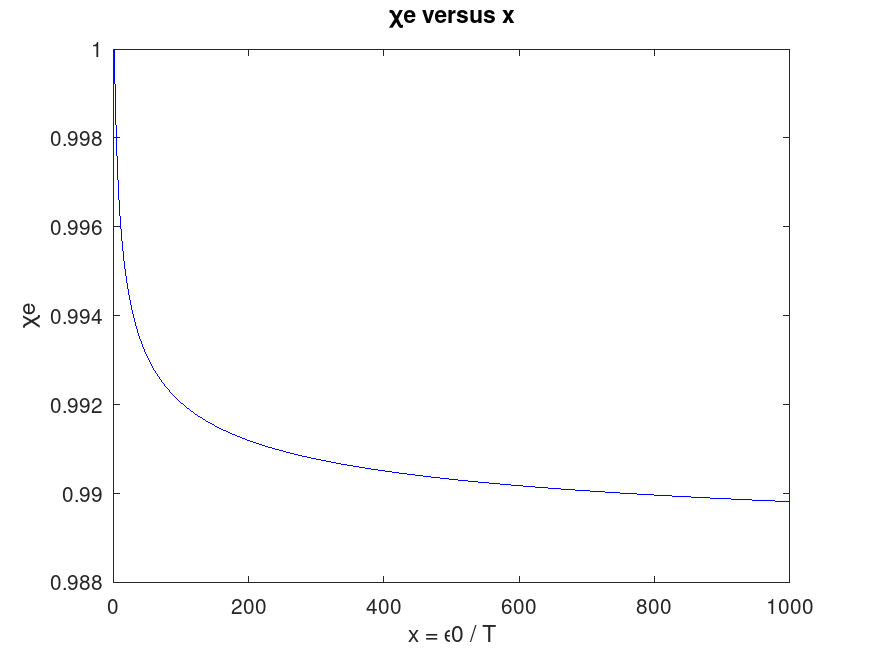
\includegraphics[width=.7\textwidth]{Figure}
          \label{fig:1}
        \end{figure}

        We may observe that, since $x$ is inversely related to the temperature, the plot takes on the inverse shape of that of the Saha solution, as expected.

    \end{enumerate}

\end{enumerate}

\end{document}

